% subject: コンピュータサイエンス第一期末試験(雛形)
% date:    18/11/21
% LaTeX2e: Japanese

\documentclass[12pt]{article}
\pagestyle{empty}
\usepackage{ascmac}
\usepackage[dvips]{epsfig}

% local.mac

%%% STYLE PARAM.s (for A4) %%%
\textwidth=16cm
\textheight=240mm

\topmargin=0mm
\headsep=0cm
\headheight=0cm
\oddsidemargin=0cm
\evensidemargin=0cm
\marginparwidth=0cm

\footnotesep=15pt
%\footheight=1.5cm
%\footskip=1.5cm

\itemsep=0.1pt
\parindent=11pt

\def\baselinestretch{1.15}

%%% LOCAL MACRO DEF.s %%%

\newcommand{\OMIT}[1]{}

% Print control (skips)
%\newcommand{\bigskip}{\vskip12pt}
%\newcommand{\medskip}{\vskip6pt}
%\newcommand{\smallskip}{\vskip3pt}
\newcommand{\paragraphskip}{\vskip\topsep}

% Itemization, etc
\newcommand{\nitem}[1]{%
\par\noindent\hangindent20pt%
\hskip20pt\llap{#1~}}
\newcommand{\nnitem}[1]{%
\par\noindent\hangindent30pt%
\hskip30pt\llap{#1~}}

\begin{document}
\noindent
\hfill{\small 20.Nov.2019}

\noindent
\hfil
{\large\bf
コンピュータサイエンス第1\textemdash 期末試験 CS4b\textemdash}
\hfil

\paragraphskip\noindent
※答案用紙は各問ごとに 1 枚使用して書くこと.\\
※答案用紙には各枚ごとに学籍番号と氏名を書くこと.

\paragraphskip
\nitem{\bf 問1.}(配点 15 点)\\
下の出力例は Python 処理系で文字列をアスキーコードに変換して出力した結果である.
この結果を参考に以下の問いに答えよ.
  \begin{itembox}{出力例}
    \begin{verbatim}
>>> list("You scream".encode("ascii"))
[89, 111, 117, 32, 115, 99, 114, 101, 97, 109]
    \end{verbatim}
  \end{itembox}
\nitem{(1)}
下図は文字列が配列に格納されている様子を示している.出力例を参考に図の (1)-(10) を 10 進表記で埋めよ.
\nitem{(2)}
各 10 進表記を 2 進表記に変換し順番に図の (11)-(20) を埋めよ.
  \begin{center}
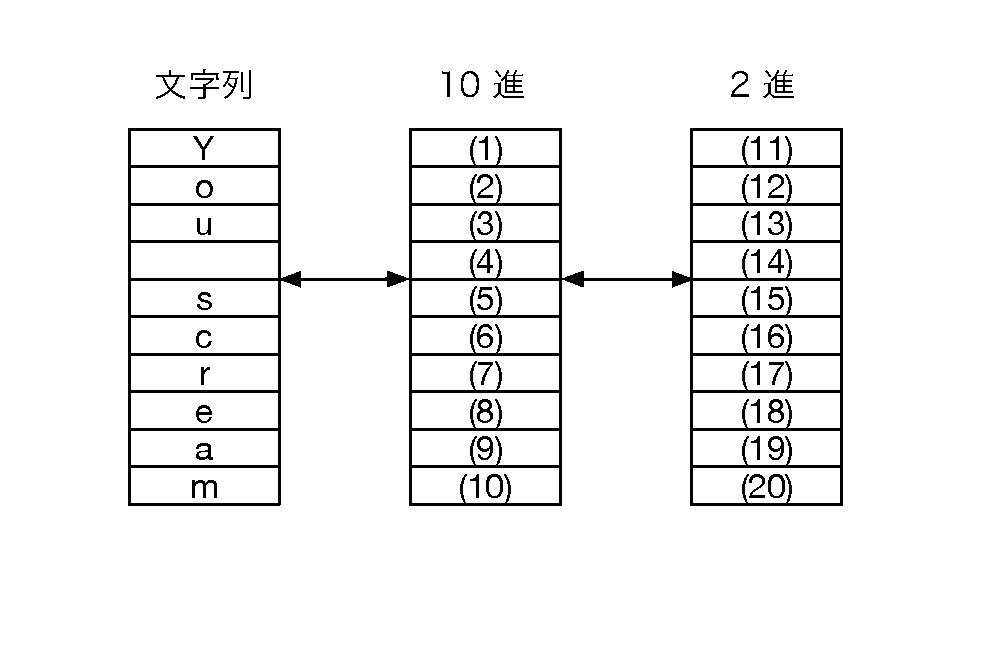
\includegraphics[scale=.9]{./Figure/elementaryCS-figStrings_hole_you_scream.eps}
  \end{center}

\hfill{裏面につづく}
\newpage
\paragraphskip
\nitem{\bf 問2.}(配点 20 点)\\
次に示したソースコードは言語 Python で書かれた Vigenere 暗号のプログラムである.
このプログラムについて以下の問いに答えよ.
\begin{itembox}{ソースコード}
\begin{verbatim}
# Vigenere Chipher
# Mode: Python3

import os

### Global variables
ALPHABET = range(ord('a'), ord('z')+1)

def letter2index (letter):
  return(letter - ALPHABET[0])
def index2letter (index):
  return(index + ALPHABET[0])
def transform(char,key):
  index = letter2index(char)
  c_index = (index + (letter2index(key))) % len(ALPHABET)
  return(index2letter(c_index))
def vigenere (key,message):
  cipher_text = message.copy()
  for i in range(len(message)):
    if message[i] in ALPHABET:
       cipher_text[i] = transform(message[i],key[i % len(key)])
    else:
       cipher_text[i] = message[i]
  return(cipher_text)
def encipher(key, message):
  letters = list(message.encode("ascii"))
  keys = list(key.encode("ascii"))
  return(bytes(vigenere(keys,letters)).decode("ascii"))

### TEST HARNESS
os.system("clear")
print(encipher("vigenere", input()))
\end{verbatim}
\end{itembox}
\nitem{(1)}
平文 "elementaryCS" が入力として与えられたときの暗号文を示せ.
\nitem{(2)}
文字の置き換えをどのようにしているか暗号化鍵と計算式を示しながら説明せよ.

\end{document}
